\documentclass[12pt]{article}
% \documentclass{elsarticle} %A different option for format styling...

%NOTE: Use of this template is *totally optional* -- it is just provided to make your life easier. If it does not do that, feel free to use your own template. The formatting does not count for points, only the answers in a readable (LaTeX-generated) format count. 

\textwidth 6.5in
\oddsidemargin 0.0in %this is a 1-inch margin
\evensidemargin 1.0in %matching 1-inch margin

\usepackage{amssymb}
\usepackage{alltt}
\usepackage{multicol}
\usepackage{hyperref}
\usepackage{mathrsfs} %for \mathscr{} 
\usepackage{amsthm}
\usepackage{amsmath}
\usepackage{listings}
\usepackage{gensymb} %for \degree
\usepackage{longtable} %for longtabu
\usepackage{hhline} %for double \hline in longtabu
\usepackage{blindtext}
\usepackage{xcolor}
\usepackage{multirow}
\usepackage{tikz}
\usetikzlibrary{shapes.misc, positioning}
\usetikzlibrary{arrows.meta}
\usepackage{graphicx}


\newtheorem{defin}{Definition}
\newtheorem{intuit}{Intuition}

%Here are the commands included in elsarticle style:
\newtheorem{thm}{Theorem}
\newtheorem{lem}[thm]{Lemma}

\interfootnotelinepenalty=10000

\renewcommand{\phi}{\varphi}
\newcommand{\always}{\Box}
\newcommand{\eventually}{\Diamond}
\newcommand{\calL}{{\cal L}}

\newcommand{\pspic}[2]{\scalebox{#1}{\includegraphics{#2}}}

% numeric sets
\newcommand{\Reals}{\mathbb{R}}      % real numbers
\newcommand{\Naturals}{\mathbb{N}}   % natural numbers
\newcommand{\Integers}{\mathbb{Z}}   % integer numbers
\newcommand{\Rationals}{\mathbb{Q}}  % rational numbers
\newcommand{\Complexes}{\mathbb{C}}  % complex numbers

% logic
\newcommand{\yields}{\vdash}         % yields
\newcommand{\proves}{\vdash}         % proves
\newcommand{\then}{\rightarrow}      % implication
\newcommand{\logeq}{\Leftrightarrow} % logically equivalent
\newcommand{\xor}{\oplus}            % xor

% formal logic
\newcommand{\Models}{\vDash}                 % models
\newcommand{\Always}{\Box}                   % always
\newcommand{\Eventually}{\lozenge}           % eventually
\newcommand{\Next}{\mathcal{X}}              % ne[X]t
\newcommand{\Until}{\ \mathcal{U}}         % [U]ntil
\newcommand{\Release}{\ \mathcal{R}}       % [R]lease
\newcommand{\WeakUntil}{\ \mathcal{W}}     % [W]eak until
\newcommand{\MightyRelease}{\ \mathcal{M}} % [M]ighty release
\newcommand{\Globally}{\mathcal{G}}          % [G]lobally
\newcommand{\Finally}{\mathcal{F}}           % [F]inally
\newcommand{\ForAllPaths}{\mathcal{A}}       % for [A] paths
\newcommand{\ExistsAPath}{\mathcal{E}}       % exists a path


%Number the Exercises with one counter through multiple sections
\newcounter{ExerciseCounter}
\setcounter{ExerciseCounter}{1} %start counting at 1


%%%%%%%%%%%%%%%%%%%%%%%%%%%%%%%%%%%%%%%%%%%%%%%%%%%%%%%%
% Figure Magic
%%%%%%%%%%%%%%%%%%%%%%%%%%%%%%%%%%%%%%%%%%%%%%%%%%%%%%%%
\usepackage{epsfig}
\usepackage{float}
\usepackage{subfigure}
\usepackage{wrapfig}
\renewcommand{\topfraction}{.95} %figures can take up at most 95% of the page before being alone
\renewcommand{\bottomfraction}{.99} %figures can take up at most 99% of the page before being alone
\renewcommand{\textfraction}{.1} %at most this this % of page will be text before making figure-only page
\addtolength{\abovecaptionskip}{-3mm}


\begin{document}

\title{\bf
\large Learning Mission-time Linear Temporal Logic (MLTL) from Data}

\author{
  Zili Wang\\
  \texttt{ziliw1@iastate.edu}
  \and
  Luke Marzen\\
  \texttt{ljmarzen@iastate.edu}
  \and
  Nhan Tran\\
  \texttt{nhtran@iastate.edu}
  \and
  Swaminathan Jayaraman\\
  \texttt{swamjay@iastate.edu}
}

\date{April 26, 2024}

\maketitle

% Abstract
\begin{abstract}
  Mission-time Linear Temporal Logic (MLTL) is a discrete time, finite interval bounded variant of the popular Linear Temporal Logic (LTL). 
  Given a set of positive traces, characterizing desirable behaviors of a system, and a set of negative traces, characterizing undesirable behaviors, the goal is to learn a MLTL formula succinctly capturing the system behavior.
  In this technical report, we describe five differing approaches to MLTL inference: genetic programming, informed beam search, deep learning via transformers, template-driven search, and Bayesian network structure learning.  
\end{abstract}

\section{Introduction}



Mission-time Linear Temporal Logic (MLTL) is a discrete time, finite interval bounded temporal logic that has found numerous recent applications. 
For example, MLTL was the specification logic for NASA's Robonaut2 verification project \cite{KZJZR20}, as well as for the design-time and runtime verification of the NASA Lunar Gateway Vehicle System Manager \cite{DBR21}.
Other applications of MLTL include autonomous satellite \cite{JAXA}, UAV Traffic Management \cite{HCHJR21}, and more. 

Given a (finite) set of atomic propositions $\mathcal{AP}$, the syntax of MLTL formulas $\phi$ and $\psi$ are defined recursively: 
$$ \phi, \psi := true \ | \ false \ | \ p \ | \ \neg \phi \ | \ \phi \land \psi \ | \ \phi \lor \psi \ | \ \Finally_{[a,b]} \phi \ | \ \Globally_{[a,b]} \phi \ | \ \phi \Until_{[a,b]}\ \psi \ | \ \phi \Release_{[a,b]}\ \psi, $$
where $p \in \mathcal{AP}$, and $a, b \in \mathbb{Z}$ such that $0 \leq a \leq b$. 
The symbols $\mathcal{F},\mathcal{G},\mathcal{U},\mathcal{R}$ denote the temporal operators Future, Globally, Until, and Release, respectively.
A trace $\pi$ represents a sequence of truth assignments to the atomic propositions in $\mathcal{AP}$ over time, and $\pi$ satisfies a MLTL formula $\phi$ is denoted as $\pi \models \phi$.
If $\pi$ does not satisfy $\phi$, then $\pi \not\models \phi$.
The explicit semantics of each MLTL operator can be found in \cite{WEST-iFM23}.

The object of this proposed project is to explore various approaches to MLTL inference, formally described as follows: 
Given a set traces $T = T^+ \cup T^-$ over $n$ variables, learn a MLTL formula $\phi$ such that for all $\pi \in T^+$, $\pi \models \phi$, and for all $\pi \in T^-$, $\pi \not\models \phi$. 
Intuitively, $T^+$ represents the set of positive examples, or desirable behaviors, and $T^-$ represents the set of negative examples, or undesirable behaviors.
These traces can come from simply observing the behavior of some system of interest, or they can be generated by some other means, such as a model checker or a simulator.
The goal is to learn a MLTL formula that specifies the desired behavior of the system, and to do so in a way that generalizes to new, unseen traces.

There is a large corpus of work on learning regular languages, stemming from Angluin's $L^*$ algorithm \cite{ANGLUIN_Lstar} that learns a minimal deterministic finite automata (DFA) from positive and negative examples. Work in learning temporal logic formulas have also recently been explored, with approaches ranging from symbolic learning algorithms \cite{roy_ltlf_learning, camacho_ltlf_learning} to deep learning algorithms \cite{stl_learning, Luo_Liang_Du_Wan_Peng_Zhang_2022}.
There is no published work on learning MLTL formulas, and the goal of this project is to explore various approaches to this problem, and to compare and contrast their performance.

Previously, Zili Wang has developed and evaluated Genetic Programming (GP) based approach to learning MLTL formulas, and lays the groundwork for the proposed project.
The repository containing the code and datasets for this project can be found at 

\noindent \url{https://github.com/zwang271/mltl-inference}.
Work that will be reused includes the following components:
\begin{enumerate}
  \item A parser (Python) for MLTL formulas, that can compute various properties of the formula, such as the number of atomic propositions, the syntax tree, worst propagation delay (wpd) (defined in \cite{KZJZR20}), and various other useful functions.  
  \item An MLTL interpreter (C++): on input trace $\pi$ and a MLTL formula $\phi$, determines if $\pi \models \phi$.
  \item A dataset generator (Python) that given an MLTL formula, uses either random trace sampling or regular expression sampling (see \cite{WEST-iFM23}) to generate a set of positive and negative examples.
  \item 9 datasets, each with 500 positive and 500 negative examples, split into 80\% training and 20\% testing sets.
\end{enumerate}

As a group, we aim evaluate various approaches using a combination of metrics such as run time, formula accuracy as a percent of correctly classified traces, and formula length/complexity.  
Each team member will be responsible for implementing a different technique, though if some techniques are found to be non-viable or require more effort than reasonable to complete in a semester we will remain flexible and collaborate to ensure the project is completed.

\section{Approaches}
  
% Prior work applies Graph Neural Networks (GNN) to learn Linear Temporal Logic over finite trace (LTLf) formulas by extracting formula from the weights of trained GNNs \cite{Luo_Liang_Du_Wan_Peng_Zhang_2022}.
% The approach will be adapted to MLTL, and we seek generalize the methodology in interesting ways. 
% For example, we may explore the use of different GNN architectures, or applying deep reinforcement learning techniques to a game playing reformulation of the problem.

\subsection{Transformer Neural Network}
	
% Transformer Neural Network is a neural network technique used to process sequences. Transformers are popular in Natural Language Processing for their ability to identify context in text and parallel processing. In terms of this project, transformer will be used for its Self-attention mechanisms to identify the relationship between each trace in the MLTL traces and its formula. The input to the transformer will be the negative and positive MLTL traces. The output will be the MLTL formula.

\subsection{Template Driven Search}
	
% A template-driven approach for MLTL inference uses predefined formula templates to guide the search for an MLTL formula consistent with given positive and negative traces. In this project, candidate MLTL formulas will be systematically generated by filling template placeholders through an automated search mechanism, prioritizing the efficiency of the search process. Each candidate is then evaluated against a set of positive and negative traces. Formula selection will be performed based on additional considerations such as simplicity and generalizability to ensure practical utility.

\subsection{Beam Search}

% This approach will formulate MLTL inference into a search problem then apply A*.  Multiple heuristic functions will be evaluated and compared.  Heuristic functions may consider factors such as accuracy against positive and negative traces and length or complexity of the formula.  Due to the search space growing exponentially as formula length increases it will likely be necessary to employ inadmissible heuristics which could greatly accelerate the search but could result in suboptimal solutions.  An analysis will be conducted to assess the trade-offs between execution time and solution optimality using admissible versus inadmissible heuristic functions.

\textit{Beam Search} is a variant of best-first search that uses breadth-first search to explore the next layer of the search tree, but limits the number of successors to a predetermined amount $b$, known as the \textit{beam width}. Beam search with an infinite beam width would be equivalent to best-first search. At each level, all successor nodes are generated and sorted by a heuristic cost function, $h$. Only the $b$ candidate nodes with the lowest cost are kept, and all other nodes are discarded. This limits memory usage and maintains tractability for large state space problems, such as MLTL-inference. The primary disadvantage of beam search is the possibility of pruning all paths to the optimal goal state.

\subsubsection{Search Problem Formulation}

This section details the search problem formulation we used to reduce MLTL-inference to a search problem.

\textit{State Space} -- The space of possible MLTL formulas is constructed recursively from the given alphabet of propositions and operators.
\[
\phi, \psi := true \ | \ false \ | \ p \ | \ \neg \phi \ | \ \phi \land \psi \ | \ \phi \lor \psi \ | \ \Finally_{[a,b]} \phi \ | \ \Globally_{[a,b]} \phi \ | \ \phi \Until_{[a,b]} \psi \ | \ \phi \Release_{[a,b]} \psi
\]

\textit{Initial State} -- The empty formula.

\textit{Goal State} -- A formula that best describes the given positive and negative traces, according to evaluation criteria that include accuracy and simplicity.

\textit{Actions} -- Operations can be applied to a current formula to generate new candidate formula. This includes adding a new operator, modifying an existing operator, or combining multiple formulas.

\textit{Cost Function} -- The cost of a node is considered to be $1-accuracy$, where accuracy is evaluated over all input traces in the training dataset.

\textit{Termination Criteria} -- The search should terminate once a predetermined depth, accuracy, or time-limit is reached.

\subsubsection{Implementation}

Developing heuristics to explore the enormous state space in an efficient manner proved to be very challenging. This sub-section discuss our implementation of beam search for MLTL-inference and outlines the techniques we employed to address these challenges.

Our first observation was that constructing formulas one operator and propositional variable at a time was wasteful. Consider that temporal operators often contain simple boolean function, for example, $\Finally_{[0,10]}\ (p_0 \land p_1 ) \lor (p_1 \land p_2 )$. If we construct this formula by adding one additional operator and propositional variable at each level of the search then constructing this formula would require several levels of search to be completed. Instead, we try to pre-generate \textit{interesting} boolean functions that can be considered for inclusion at any point in the search tree. Generating boolean functions is a hard problem, since for each variable there are two possible assignments and for each unique assignment of all variables there are two possible corresponding truth values. Thus the run time to enumerate all boolean function for $n$ propositional variables is double exponential, $O(2^{2^n})$. The number of boolean functions reaches the capacity of a 32-bit integer with just 5 variables. To keep this problem a reasonable size and we limit the size of boolean functions we generate to contain at most 2-4 unique variables. It is trivial to construct a boolean function in \textit{Conjunctive Normal Form} (CNF) or \textit{Disjunctive Normal Form} (DNF) given a truth table, however, this creates long formulas which counters the goal of finding concise representations. To address this we pass each boolean function through the Quine-McCluskey algorithm\cite{quine1952,quine1955,mccluskey1956} which returns an equivalent boolean function as a simplified DNF.

To determine whether a boolean function may be useful as part of the construction of MLTL formulas, we begin by evaluating each function as the operand to the Finally and Globally operators over all training traces. If the boolean function as an operand to one of these two unary temporal operators achieves an accuracy of over 50\% then we consider it to be \textit{interesting}, otherwise we will discard it. We also always consider all variables are on their own to be \textit{interesting} since this allows us to construct functions that we may have prematurely dismissed. We also discard boolean expressions that even when simplified are very long. 

Iterating over every possible combination of bounds for each operator can quickly make this problem intractable, so we fix the amount that the bounds can be stepped to some fraction of the average trace length. In general using approximate bounds can still result in accurate formulas as long as the structure and operators of the formula are correct. By giving up precision on the operator bounds we can identify the correct structure and operators in a practical amount of time. After identifying the correct formula structure another algorithm could be used to optimize the operator bounds.

In our implementation each depth of the search tree is defined by the number of nested temporal operators. As a result most practical MLTL formulas will be found at depths 1 to 3. To build formulas of the next level we use already explored formulas of the highest accuracy as operands to new formulas. This heuristic tends to lead towards good solutions, but can sometimes make the optimal solution unreachable, hence this is an inadmissible heuristic.

After all the above heuristics and simplifying assumptions, the problem can now be computed in a reasonable amount of time. Exploring each subsequent level of the search tree is now mainly limited by evaluation time. Since the evaluation of each formula can be done independently of any other formula, this is embarrassingly parallel. As such we have paralyzed the algorithm to run across all available CPU cores.

\subsection{MLTL formulas as Bayesian Networks}

Originally, the idea was to define a correspondance between MLTL formulas and Bayesian Networks. 
Then we would leverage the many techniques for learning structure of Bayesian Networks from data interpret a learned Bayesian Network as a MLTL formula. 
The first step was succesful, and the details of the correspondance are outlined below.
However, we were not able to formulate a well defined structure learning problem that would allow us to extract a MLTL formula from a learned Bayesian Network. 
We also give a discussion of the challenges encountered with this second step, and potential future work.

\subsubsection{Correspondance between MLTL formulas and Bayesian Networks}

The correspondance between MLTL formulas and Bayesian Networks is recursively defined.

\begin{figure}[h]
\centering
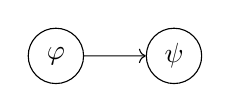
\begin{tikzpicture}
% Define styles
\tikzstyle{node} = [rounded rectangle, draw, fill=white, text centered, minimum height=2em]
% Define nodes
\node[node] (phi) at (0,0) {$\phi$};
\node[node] (psi) at (1.5,0) {$\psi$};
% Connect the nodes
\draw[->] (phi) -- (psi);
\end{tikzpicture}
\caption{Bayesian Network structure for $\psi = \phi$ and $\psi = \neg \phi$}
\end{figure}


\begin{figure}[h]
\centering
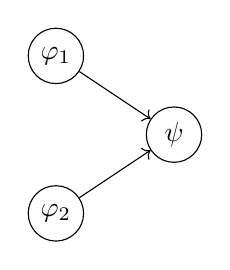
\begin{tikzpicture}
% Define styles
\tikzstyle{node} = [rounded rectangle, draw, fill=white, text centered, minimum height=2em]
% Define nodes
\node[node] (phi1) at (0,0) {$\phi_1$};
\node[node] (phi2) at (0,-2) {$\phi_2$};
\node[node] (psi) at (1.5,-1) {$\psi$};
% Connect the nodes
\draw[->] (phi1) -- (psi);
\draw[->] (phi2) -- (psi);
\end{tikzpicture}
\caption{Bayesian Network structure for $\psi = \phi_1 \land \phi_2$ and $\psi = \phi_1 \lor \phi_2$}
\end{figure}


\begin{figure}[h]
\centering
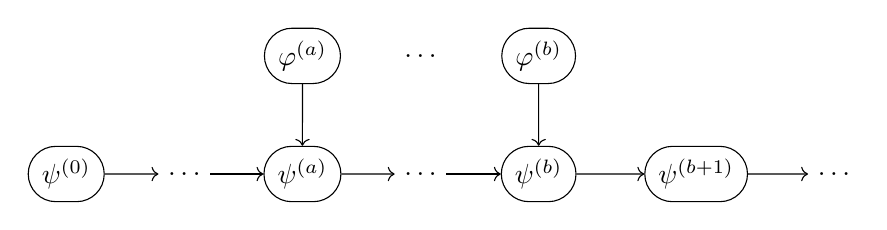
\begin{tikzpicture}
% Define styles
\tikzstyle{node} = [rounded rectangle, draw, fill=white, text centered, minimum height=2em]
% Define nodes
\node[node] (psi_0) at (0,0) {$\psi^{(0)}$};
\node (ldots0) at (1.5,0) {$\ldots$};
\node[node] (psi_a) at (3,0) {$\psi^{(a)}$};
\node[node] (phi_a) at (3,1.5) {$\phi^{(a)}$};
\node (ldots1) at (4.5,0) {$\ldots$};
\node (ldots2) at (4.5,1.5) {$\ldots$};
\node[node] (psi_b) at (6,0) {$\psi^{(b)}$};
\node[node] (phi_b) at (6,1.5) {$\phi^{(b)}$};
\node[node] (psi_b+1) at (8,0) {$\psi^{(b+1)}$};
\node (ldots3) at (9.75,0) {$\ldots$};
% Connect the nodes
\draw[->] (psi_0) -- (ldots0);
\draw[->] (ldots0) -- (psi_a);
\draw[->] (psi_a) -- (ldots1);
\draw[->] (ldots1) -- (psi_b);
\draw[->] (psi_b) -- (psi_b+1);
\draw[->] (psi_b+1) -- (ldots3);
\draw[->] (phi_a) -- (psi_a);
\draw[->] (phi_b) -- (psi_b);
\end{tikzpicture}
\caption{Bayesian Network structure for $\psi = \mathcal{F}_{[a,b]} \phi$ and $\psi = \mathcal{G}_{[a,b]} \phi$}
\end{figure}


\begin{figure}[h]
\centering
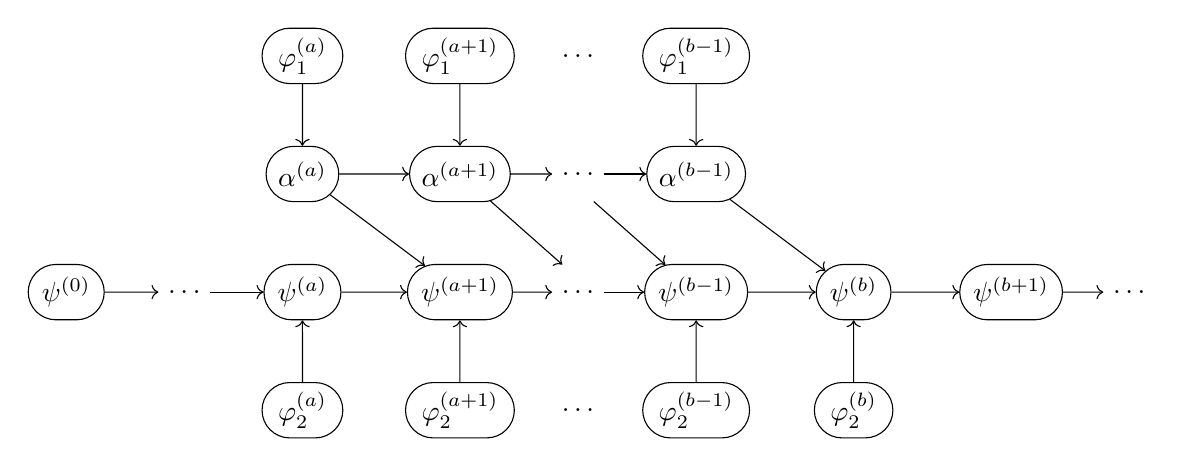
\begin{tikzpicture}
% Define styles
\tikzstyle{node} = [rounded rectangle, draw, fill=white, text centered, minimum height=2em]
% Define nodes
\node[node] (psi_0) at (0,0) {$\psi^{(0)}$};
\node (psi_ldots0) at (1.5,0) {$\ldots$};
\node[node] (psi_a) at (3,0) {$\psi^{(a)}$};
\node[node] (psi_a+1) at (5,0) {$\psi^{(a+1)}$};
\node (psi_ldots1) at (6.5,0) {$\ldots$};
\node[node] (psi_b-1) at (8,0) {$\psi^{(b-1)}$};
\node[node] (psi_b) at (10,0) {$\psi^{(b)}$};
\node[node] (psi_b+1) at (12,0) {$\psi^{(b+1)}$};
\node (psi_ldots2) at (13.5,0) {$\ldots$};
\node[node] (alpha_a) at (3,1.5) {$\alpha^{(a)}$};
\node[node] (alpha_a+1) at (5,1.5) {$\alpha^{(a+1)}$};
\node (alpha_ldots1) at (6.5,1.5) {$\ldots$};
\node[node] (alpha_b-1) at (8,1.5) {$\alpha^{(b-1)}$};
\node[node] (phi1_a) at (3,3) {$\phi_1^{(a)}$};
\node[node] (phi1_a+1) at (5,3) {$\phi_1^{(a+1)}$};
\node (phi1_ldots1) at (6.5,3) {$\ldots$};
\node[node] (phi1_b-1) at (8,3) {$\phi_1^{(b-1)}$};
\node[node] (phi2_a) at (3,-1.5) {$\phi_2^{(a)}$};
\node[node] (phi2_a+1) at (5,-1.5) {$\phi_2^{(a+1)}$};
\node (phi2_ldots1) at (6.5,-1.5) {$\ldots$};
\node[node] (phi2_b-1) at (8,-1.5) {$\phi_2^{(b-1)}$};
\node[node] (phi2_b) at (10,-1.5) {$\phi_2^{(b)}$};

% Connect the nodes
\draw[->] (psi_0) -- (psi_ldots0);
\draw[->] (psi_ldots0) -- (psi_a);
\draw[->] (psi_a) -- (psi_a+1);
\draw[->] (psi_a+1) -- (psi_ldots1);
\draw[->] (psi_ldots1) -- (psi_b-1);
\draw[->] (psi_b-1) -- (psi_b);
\draw[->] (psi_b) -- (psi_b+1);
\draw[->] (psi_b+1) -- (psi_ldots2);
\draw[->] (alpha_a) -- (psi_a+1);
\draw[->] (alpha_a+1) -- (6.3,0.35);
\draw[->] (6.7,1.15) -- (psi_b-1);
\draw[->] (alpha_b-1) -- (psi_b);
\draw[->] (alpha_a) -- (alpha_a+1);
\draw[->] (alpha_a+1) -- (alpha_ldots1);
\draw[->] (alpha_ldots1) -- (alpha_b-1);
\draw[->] (phi1_a) -- (alpha_a);
\draw[->] (phi1_a+1) -- (alpha_a+1);
\draw[->] (phi1_b-1) -- (alpha_b-1);
\draw[->] (phi2_a) -- (psi_a);
\draw[->] (phi2_a+1) -- (psi_a+1);
\draw[->] (phi2_b-1) -- (psi_b-1);
\draw[->] (phi2_b) -- (psi_b);

\end{tikzpicture}
\caption{Bayesian Network structure for $\psi = \phi_1 \mathcal{U}_{[a,b]} \phi_2$}
\end{figure}

\begin{figure}[h]
\centering
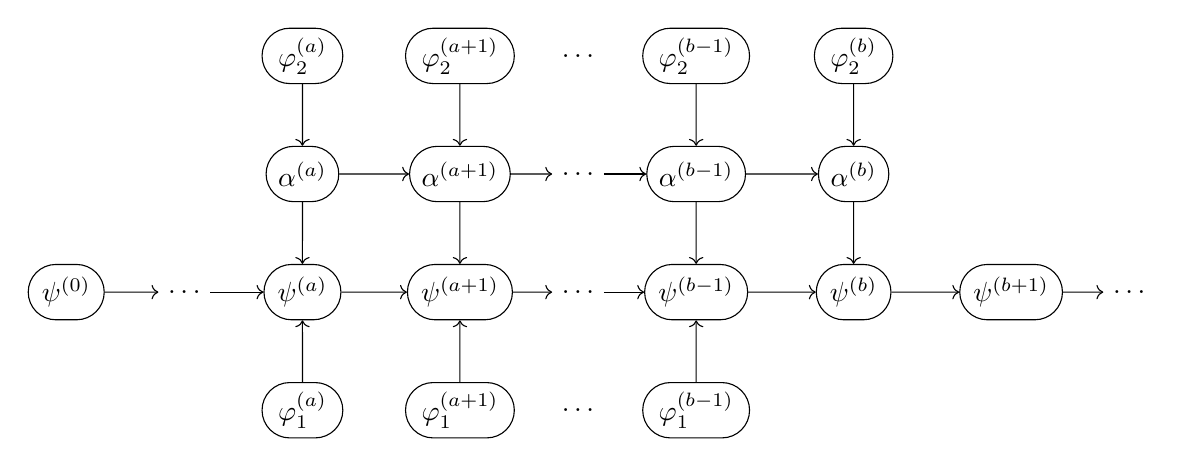
\begin{tikzpicture}
% Define styles
\tikzstyle{node} = [rounded rectangle, draw, fill=white, text centered, minimum height=2em]
% Define nodes
\node[node] (psi_0) at (0,0) {$\psi^{(0)}$};
\node (psi_ldots0) at (1.5,0) {$\ldots$};
\node[node] (psi_a) at (3,0) {$\psi^{(a)}$};
\node[node] (psi_a+1) at (5,0) {$\psi^{(a+1)}$};
\node (psi_ldots1) at (6.5,0) {$\ldots$};
\node[node] (psi_b-1) at (8,0) {$\psi^{(b-1)}$};
\node[node] (psi_b) at (10,0) {$\psi^{(b)}$};
\node[node] (psi_b+1) at (12,0) {$\psi^{(b+1)}$};
\node (psi_ldots2) at (13.5,0) {$\ldots$};
\node[node] (alpha_a) at (3,1.5) {$\alpha^{(a)}$};
\node[node] (alpha_a+1) at (5,1.5) {$\alpha^{(a+1)}$};
\node (alpha_ldots1) at (6.5,1.5) {$\ldots$};
\node[node] (alpha_b-1) at (8,1.5) {$\alpha^{(b-1)}$};
\node[node] (alpha_b) at (10,1.5) {$\alpha^{(b)}$};
\node[node] (phi2_a) at (3,3) {$\phi_2^{(a)}$};
\node[node] (phi2_a+1) at (5,3) {$\phi_2^{(a+1)}$};
\node (phi2_ldots1) at (6.5,3) {$\ldots$};
\node[node] (phi2_b-1) at (8,3) {$\phi_2^{(b-1)}$};
\node[node] (phi2_b) at (10,3) {$\phi_2^{(b)}$};
\node[node] (phi1_a) at (3,-1.5) {$\phi_1^{(a)}$};
\node[node] (phi1_a+1) at (5,-1.5) {$\phi_1^{(a+1)}$};
\node (phi1_ldots1) at (6.5,-1.5) {$\ldots$};
\node[node] (phi1_b-1) at (8,-1.5) {$\phi_1^{(b-1)}$};
% Connect the nodes
\draw[->] (psi_0) -- (psi_ldots0);
\draw[->] (psi_ldots0) -- (psi_a);
\draw[->] (psi_a) -- (psi_a+1);
\draw[->] (psi_a+1) -- (psi_ldots1);
\draw[->] (psi_ldots1) -- (psi_b-1);
\draw[->] (psi_b-1) -- (psi_b);
\draw[->] (psi_b) -- (psi_b+1);
\draw[->] (psi_b+1) -- (psi_ldots2);
\draw[->] (alpha_a) -- (psi_a);
\draw[->] (alpha_a+1) -- (psi_a+1);
\draw[->] (alpha_b-1) -- (psi_b-1);
\draw[->] (alpha_b) -- (psi_b);
\draw[->] (phi2_a) -- (alpha_a);
\draw[->] (phi2_a+1) -- (alpha_a+1);
\draw[->] (phi2_b-1) -- (alpha_b-1);
\draw[->] (phi2_b) -- (alpha_b);
\draw[->] (phi1_a) -- (psi_a);
\draw[->] (phi1_a+1) -- (psi_a+1);
\draw[->] (phi1_b-1) -- (psi_b-1);
\draw[->] (alpha_a) -- (alpha_a+1);
\draw[->] (alpha_a+1) -- (alpha_ldots1);
\draw[->] (alpha_ldots1) -- (alpha_b-1);
\draw[->] (alpha_b-1) -- (alpha_b);


\end{tikzpicture}
\caption{Bayesian Network structure for $\psi = \phi_1 \mathcal{R}_{[a,b]} \phi_2$}
\end{figure}

\newpage
\section{Evaluation}

\subsection{Datasets}

{\footnotesize
\centering
\begin{tabular}{llrrr}
Dataset            & Generating Formula                                         & \begin{tabular}[c]{@{}l@{}}Formula\\ Size\end{tabular} & \begin{tabular}[c]{@{}l@{}}Num.\\ Variables\end{tabular} & \begin{tabular}[c]{@{}l@{}}Avg. Trace\\ Length\end{tabular} \\
basic\_future      & $\Finally_{[0,10]}(p_0 \lor p_1)$                                         & 4                                                      & 2                                                         & 14.9                                                        \\
basic\_global      & $\Globally_{[0,10]}(p_0 \land p_1 \land \neg p_2)$                                   & 7                                                      & 3                                                         & 14.6                                                        \\
basic\_release     & $p_0 \Release_{[0,10]}\ p_2$                                            & 3                                                      & 3                                                         & 14.0                                                        \\
basic\_until       & $p_1 \Until_{[0,10]}\ p_2$                                            & 3                                                      & 3                                                         & 14.0                                                        \\
fmsd17\_formula1   & $\Globally_{[0,10]}\neg (\neg p_0 \land \neg (p_1 \Until_{[0,10]}\ p_0))$                         & 9                                                      & 2                                                         & 24.0                                                        \\
fmsd17\_formula2   & $\Globally_{[0,99]}\neg (p_6 \land \neg ((\neg p_2 \land \neg p_3 \land \neg p_4) \Until_{[0,99]}\ p_5))$     & 15                                                     & 7                                                         & 23.9                                                        \\
fmsd17\_formula3   & $\Globally_{[0,99]}(p_4 \land p_5 \land p_6)$                                   & 6                                                      & 7                                                         & 14.0                                                        \\
nasa-atc\_formula1 & $\Globally_{[0,10]}\neg (\neg p_0 \land \neg (p_1 \Until_{[0,10]}\ p_0))$                         & 9                                                      & 2                                                         & 23.9                                                        \\
nasa-atc\_formula2 & $\Globally_{[0,99]}\neg (p_6 \land \neg ((\neg p_2 \land \neg p_3 \land \neg p_4) \Until_{[0,99]}\ p_5))$     & 15                                                     & 7                                                         & 23.9                                                        \\
rv14\_formula1     & $\Globally_{[0,99]}\neg (p_1 \land (\texttt{tt} \Until_{[0,30]}\ p_0) \land (\texttt{tt} \Until_{[0,99]}\ p_2))$ & 11                                                     & 3                                                         & 14.0                                                        \\
rv14\_formula2     & $\Globally_{[0,99]}\neg (\neg p_0 \land \neg (p_1 \Until_{[0,30]}\ p_0))$                      & 9                                                      & 2                                                         & 14.1                                                       
\end{tabular}
}

\subsection{Results}

\subsubsection{Beam Search}


{\footnotesize
\centering
\begin{tabular}{llrrr}
Dataset                             & Best Formula(s) Found                                                                                   & \begin{tabular}[c]{@{}l@{}}Formula\\ Size\end{tabular} & \begin{tabular}[c]{@{}l@{}}Compute\\ Time (s)\end{tabular} & \begin{tabular}[c]{@{}l@{}}Formula\\ Accuracy\end{tabular} \\
basic\_future                       & $\Finally_{[0,10]}(p_1 \lor p_0)$                                                                                 & 4                                                      & 0.1                                                        & 100\%                                                      \vspace{0.5em}\\
basic\_global                       & $\Globally_{[0,10]}(p_0 \land p_1 \land \neg p_2)$                                                                           & 7                                                      & 0.2                                                        & 100\%                                                      \vspace{0.5em}\\
basic\_release                      & $p_0 \Release_{[0,10]}\ p_2$                                                                                    & 3                                                      & 0.2                                                        & 100\%                                                      \vspace{0.5em}\\
basic\_until                        & $p_1 \Until_{[0,10]}\ p_2$                                                                                    & 3                                                      & 0.2                                                        & 100\%                                                      \vspace{0.5em}\\
fmsd17\_formula1                    & $\Globally_{[0,10]}(p_1 \Until_{[0,15]}\ p_0)$                                                                           & 4                                                      & 1.4                                                        & 100\%                                                      \vspace{0.5em}\\
\multirow{2}{*}{fmsd17\_formula2}   & $\Globally_{[0,10]}(((\neg p_6 \lor p_5) \Until_{[0,15]}\ (\neg p_2 \land \neg p_3)) \lor \neg p_6 \lor p_5)$                                             & 16                                                     & 13.3                                                       & 98.2\%\ \ \\
                                    & \begin{tabular}[c]{@{}l@{}}$\Globally_{[0,10]}((\neg p_6 \Until_{[0,5]}\ p_5) \lor \neg p_6 \lor \neg p_4)$ \\ \hspace{2em}$\Release_{[0,10]}\ \Globally_{[0,10]}(((\neg p_6 \lor p_5) \Until_{[0,5]}\ (\neg p_2 \land \neg p_3)) \lor \neg p_6 \lor p_5)$\end{tabular} & 28                                                     & 138.9                                                      & 99.4\%                                                     \vspace{0.5em}\\
fmsd17\_formula3                    & $\Globally_{[0,10]}(p_4 \land p_5 \land p_6)$                                                                            & 6                                                      & 19.4                                                       & 100\%                                                      \vspace{0.5em}\\
nasa-atc\_formula1                  & $\Globally_{[0,10]}(p_1 \Until_{[0,10]}\ p_0)$                                                                           & 4                                                      & 2.3                                                        & 100\%                                                      \vspace{0.5em}\\
\multirow{2}{*}{nasa-atc\_formula2} & $\Globally_{[0,10]}(((\neg p_6 \lor p_5) \Until_{[0,10]}\ (\neg p_2 \land \neg p_3)) \lor \neg p_6 \lor p_5)$                                             & 16                                                     & 21.8                                                       & 97.6\%\ \                                                      \\
                                    &    \begin{tabular}[c]{@{}l@{}}$\Globally_{[0,10]}(((\neg p_6 \lor \neg p_4) \Until_{[0,5]}\ p_5) \lor \neg p_6)$ \\ \hspace{2em} $\Release_{[0,10]}\ \Globally_{[0,10]}((\neg p_2 \land \lor p      _3) \Until_{[0,5]} (\neg p_6 \lor p_5))$\end{tabular}                  & 23                                                     & 4022.4                                                     & 99.2\%                                                     \vspace{0.5em}\\
\multirow{2}{*}{rv14\_formula1}     & $\Globally_{[0,10]}((p_1 \Release_{[0,5]}\ (\neg p_2 \lor \neg p_0)) \lor \neg p_1)$                                                           & 11                                                     & 2.3                                                        & 100\% \                                                     \\
                                    & $\Globally_{[0,10]}(\neg p_2 \lor \neg p_1 \lor \neg p_0)$                                                                         & 9                                                      & 3.3                                                        & 100\%                                                      \vspace{0.5em}\\
rv14\_formula2                      & $\Globally_{[0,10]}((p_0 \land p_1) \Until_{[0,5]}\ p_0)$                                                                     & 6                                                      & 0.8                                                        & 100\%\ \                                                      
\end{tabular}
}

\section{Conclusion}


\section{Statement of Contributions}
% To ensure that each team member gets credit for his or her
% contributions, the final report should include a statement of contributions that explicitly
% identifies the contributions of each team member and a statement that every team
% member concurs with the contents of the report.

Throughout this project, all team members have consistently collaborated, from the initial brainstorming of approaches to discussions of challenges encountered and potential solutions. The project's workload was divided in a manner that allowed each team member to leverage their expertise and interests to explore the feasibility of a different approach. The notable contributions of each team member are outlined below.



\textit{Zili Wang} -- 

\textit{Luke Marzen} -- Contributed the beam search based solution for the MLTL-inference problem. Wrote a working multi-threaded beam search implementation in C++ and evaluated its performance. Implemented the Quine-McCluskey algorithm to generate simplified DNF boolean functions.

\textit{Nhan Tran} -- 

\textit{Swaminathan Jayaraman} -- 


\newpage
\bibliographystyle{plain} % We choose the "plain" reference style
\bibliography{Citations} % Entries are in the refs.bib file
\end{document}
